% !TEX root = ..\thesis.tex

\chapter{CƠ SỞ LÍ THUYẾT}

% các cách sử dụng để giải quyết bài toán
\section{Bài toán phân loại ảnh và kỹ thuật học sâu (Deep learning)}
Phân loại ảnh là một bài toán phổ biến trong lĩnh vực thị giác maý tính. Mục tiêu của bài toán là làm cho máy tính có khả năng xác định nhãn của hình ảnh. Cụ thể hơn bài toán có đầu vào và đầu ra như sau:

- Đầu vào: Ảnh chứa đối tượng cần xác định nhãn và danh sách các nhãn (labels).

- Đầu ra: nhãn tương ứng với đối tượng trong ảnh đầu vào.

% kiếm đại hình phân loại ảnh nào cũng được, có liên quan đến đề tài càng tốt
Bài toán này được áp dụng trong nhiều lĩnh vực như: phân loại biển báo giao thông, phân loại chữ viết tay,... Các phương pháp giải quyết bài toán được chia làm hai loại: tiếp cận dựa trên máy học truyền thống và học sâu. Đối với cách tiếp cận dựa trên máy học trước tiên cần phải xác định các đặc trưng từ hình ảnh bằng một số phương pháp như: Scale-invariant feature transform (SIFT), Histogram of oriented gradients (HOG). Sau đó sử dụng thêm một số kỹ thuật phân lớp như thuật toán Support vector machine (SVM) hoặc Decision Tree để phân loại đối tượng. 

Cách tiếp cận dựa trên học sâu sử dụng kiến trúc mạng Convolution neural network cho cả việc trích xuất đặc trưng và phân loại đối tượng. Ngoài ra ta có thể kết hợp cả hai phương pháp bằng cách sử dụng mạng Convolution neural network để trích xuất đặc trưng sau đó sử dụng các kỹ thuật phân lớp để phân loại đối tượng. 

Trong những năm gần đây, sự phát triển của khoa học kỹ thuật và lượng dữ liệu ngày càng lớn đã tạo điều kiện cho các kiến trúc mạng CNN được áp dụng ngày càng nhiều trong việc giải quyết các bài toán phân loại ảnh. Các mô hình này cũng mang lại kết quả cao với thời gian ngắn đủ để đáp ứng yêu cầu áp dụng trong các bài toán real-time của con người. Chính vì vậy chúng tôi đã sử dụng thuật toán CNN cho khóa luận này.

\section{Kiến trúc mạng học sâu CNN}
CNN là một kiến trúc mạng bao gồm các lớp: convolution layer + nonlinear layer, pooling layer, fully connected layer liên kết với nhau theo một thứ tự nhất định. Thông thường, ảnh được truyền qua lớp convolution + nonlinear sau đó đến pooling layer. Bộ ba convolution + nonlinear và pooling layer được lặp lại nhiều lần trong mạng. Sau đó các giá trị tính toán được lan truyền qua tầng fully connected và softmax để phân loại đối tượng trong ảnh. Hình minh họa mạng CNN cơ bản.

Trong kiến trúc mạng này ảnh đầu vào được biểu diễn dưới dạng ma trận. Lớp Convolution được sử dụng để phát hiện đặc trưng cụ thể của ảnh, từ các đặc trưng cơ bản như góc, cạnh đến các đặc trưng phức tạp như texture của ảnh. Một ma trận có kích thước nhỏ (3x3 hoặc 5x5) được gọi là filter sẽ lướt qua toàn bộ ảnh từ trái sang phải và từ trên xuống dưới để phát hiện các đặc trưng trong ảnh. 

\begin{figure}
    \centering
    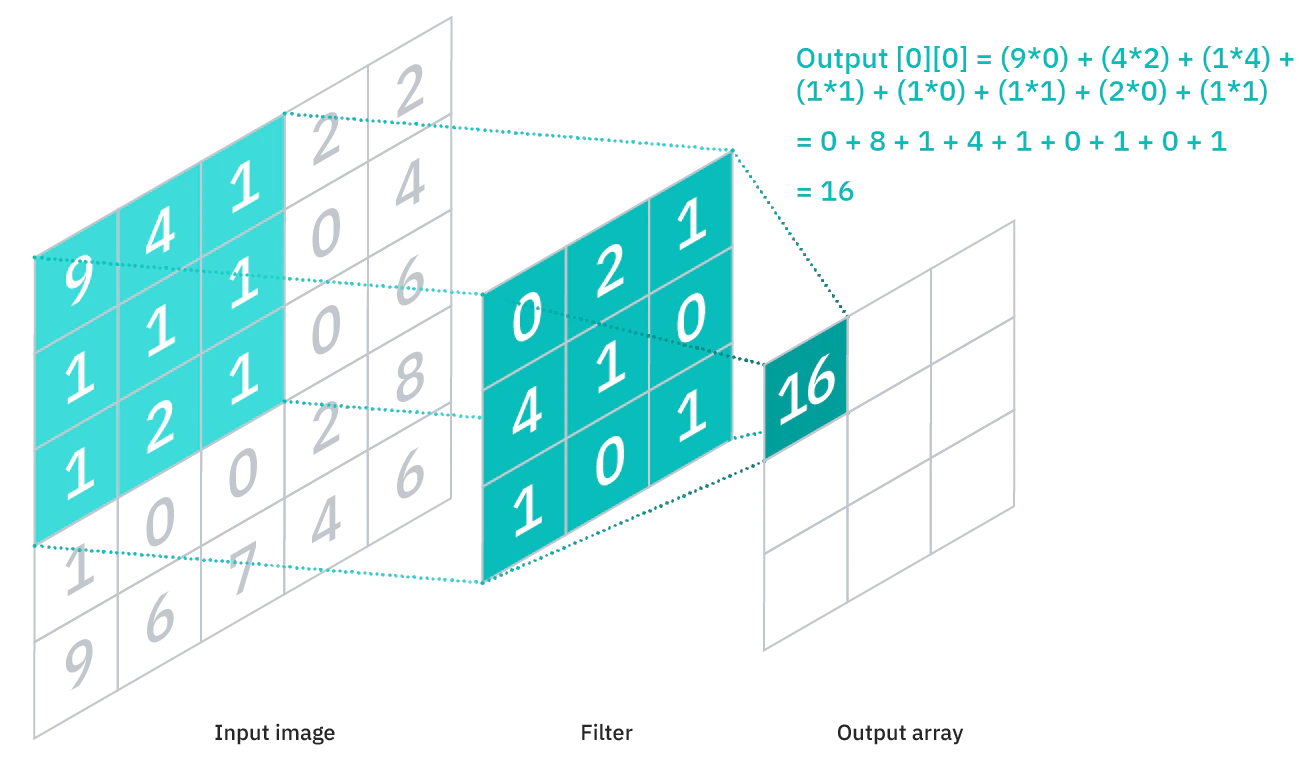
\includegraphics[width=\textwidth]{images/Quanh/cnn.png}
    \caption{Ví dụ về phép tính convoluted cho neural network} \cite{deeplearningphoton}
\end{figure}

Kích thước của filter tỉ lệ thuận với số tham số cần học và thường là số lẻ. Sau khi áp dụng phép convolution thì ma trận đầu vào sẽ nhỏ dần dẫn đến số layer của mô hình CNN bị giới hạn. Vì vậy cần phải lưu ý đến tham số stride, thể hiện số pixel cần phải dịch chuyển mỗi khi trượt filter trên ảnh và thêm padding có giá trị bằng 0 ở phần khung của ảnh. Tương tự như mạng neurald network, CNN cũng sử dụng hàm kích hoạt như ReLU hoặc tanh đặt ngay sau tầng convolution. Đối với dữ liệu ảnh hàm kích hoạt thường được sử dụng là ReLU, hàm này gán những giá trị âm bằng 0 và giữ nguyên các giá trị lớn hơn 0.

Pooling layer được xếp sau các lớp convolution để giảm tham số. Các loại pooling được sử dụng chủ yếu là max pooling và average. Các lớp này sẽ được lặp lại theo thứ tự để tạo ra feature map cuối cùng sau đó truyền vào tầng fully connected. Tầng này chuyển ma trận nhận được thành vector và phân loại vector đó tương tự như mạng neural network.

% dùng CNN giải quyết bài toán gì, lý thuyết về CNN, còn các phần khác của QUyết đưa vào mục dưới ( mục đóng góp)
% Mạng CNN là một tập hợp các lớp Convolution chồng lên nhau và sử dụng các hàm nonlinear activation như ReLU và tanh để kích hoạt các trọng số trong các node. CNN được dùng trong trong nhiều bài toán như nhân dạng ảnh, phân tích video, ảnh MRI, hoặc cho bài các bài của lĩnh vự xử lý ngôn ngữ tự nhiên. Trong đề tài này, chúng tôi đã sử dụng mạng CNN để giải quyết bài toán phân loại rác.
% Bài toán có đầu vào là một hình ảnh của rác được đưa vào thùng và đầu ra là nhãn của loại rác đó.
% CNN bao gồm tập hợp các lớp cơ bản bao gồm: convolution layer + nonlinear layer, pooling layer, fully connected layer. 
% Các lớp này liên kết với nhau theo một thứ tự nhất định. 
% Thông thường, một ảnh sẽ được lan truyền qua tầng convolution layer + nonlinear layer đầu tiên, sau đó các giá trị tính toán được sẽ lan truyền qua pooling layer, bộ ba convolution layer + nonlinear layer + pooling layer có thể được lặp lại nhiều lần trong network. Và sau đó được lan truyền qua tầng fully connected layer và softmax để tính xác suất ảnh đó chứa vật thế gì.

\label{chap:ontology}
\section{Giới thiệu TensorFlow và TensorFlow Lite}
%TensorFlow Lite is an open source deep learning framework for on-device inference.
TensorFlow Lite là giải pháp gọn nhẹ của TensorFlow cho thiết bị di động và thiết bị nhúng.
Nó cho phép suy luận học máy trên thiết bị với độ trễ thấp và kích thước nhị phân nhỏ.




\section{Giới thiệu công nghệ LoRaWan}
LoRa(long-range) sử dụng kỹ thuật điều chế gọi là Chirp Spread Spectrum.
Có thể hiểu nôm na nguyên lý này là dữ liệu sẽ được băm bằng các xung cao tần để tạo ra tín hiệu có dãy tần số cao hơn tần số của dữ liệu gốc (cái này gọi là chipped); sau đó tín hiệu cao tần này tiếp tục được mã hoá theo các chuỗi chirp signal (là các tín hiệu hình sin có tần số thay đổi theo thời gian; 
Có 2 loại chirp signal là up-chirp có tần số tăng theo thời gian và down-chirp có tần số giảm theo thời gian; và việc mã hoá theo nguyên tắc bit 1 sẽ sử dụng up-chirp, và bit 0 sẽ sử dụng down-chirp) trước khi truyền ra anten để gửi đi.

Theo Semtech công bố thì nguyên lý này giúp giảm độ phức tạp và độ chính xác cần thiết của mạch nhận để có thể giải mã và điều chế lại dữ liệu; hơn nữa LoRa không cần công suất phát lớn mà vẫn có thể truyền xa vì tín hiệu Lora có thể được nhận ở khoảng cách xa ngay cả độ mạnh tín hiệu thấp hơn cả nhiễu môi trường xung quanh.
Băng tần làm việc của LoRa từ 430MHz đến 915MHz cho từng khu vực khác nhau trên thế giới:

430MHz cho châu Á

780MHz cho Trung Quốc

433MHz hoặc 866MHz cho châu Âu

915MHz cho USA

LoRaWAN là giao thức mạng năng lượng thấp, diện rộng (LPWA) được phát triển bởi Liên minh LoRa, kết nối không dây ‘hoạt động’ với internet trong các mạng khu vực, quốc gia hoặc toàn cầu, nhắm mục tiêu các yêu cầu chính của Internet of Things (IoT) như bi thông tin liên lạc hai chiều, dịch vụ bảo mật đầu cuối, di động và nội địa hóa.
LoRaWAN sử dụng phổ không được cấp phép trong các dải ISM để xác định giao thức truyền thông và kiến ​​trúc hệ thống cho mạng trong khi lớp vật lý LoRa tạo ra các liên kết giao tiếp tầm xa giữa các cảm biến từ xa và các cổng kết nối với mạng. Giao thức này giúp thiết lập nhanh chóng các mạng IoT công cộng hoặc riêng tư ở bất cứ đâu bằng phần cứng và phần mềm.

\section{LoRa và LoRaWAN khác nhau như thể nào}

\begin{figure}[H]
    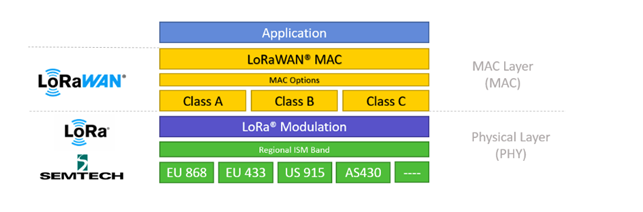
\includegraphics[width=\textwidth]{images/Quanh/LoraWan_Stack.png}
    \caption{LoRaWAN Technology Stack} \cite{lorawanoverview}
    \label{fig:lorawan_stack}
\end{figure}

Cả hai thuật ngữ thường được sử dụng đồng nghĩa, nhưng chúng có ý nghĩa khác nhau. Nhìn vào hình \ref{fig:lorawan_stack}, ta có thể thấy:
\begin{itemize}
    \item LoRa là chip (Physical layer) để giao tiếp không dây giữa Gateway và node thông qua tần số
    \item LoRaWan nằm ở MAC layer là giao thức mạng bao gồm việc sử dụng chip LoRa để liên lạc
\end{itemize}

\section{The Things Networks}
Là hệ thống bao gồm các vai trò Network Server, Application Server, join server

\subsection{Network Server}
Tư hình \ref{fig:lorawan_network}, ta suy được:
\begin{figure}[h]
    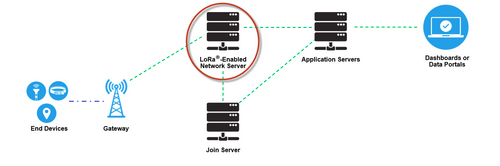
\includegraphics[width=\textwidth]{images/Quanh/LoraWan_Netwrok.png}
    \caption{Mô hình LoRaWAN Network} \cite{lorawanoverview}
    \label{fig:lorawan_network}
\end{figure}

\begin{itemize}
    \item Nhận data từ sensor của các end-devices thông qua Gateway
    \item Thực tế, các Network sẽ:
    \begin{itemize}
        \item Kiểm tra device address
        \item Đếm và quản lí số frame thực tế
    \end{itemize}
\end{itemize}

\subsection{Application Server}
Quản lí và hiển thị data, thực hiện các thao tác tạo ra down-link payload để kết nối đến end- device

\subsection{Join Network}
Trên the things network, có 2 hình thức join: OTAA ( over-the-air activation) và ABP( Activation by Personalization) có đặc điểm như bảng \ref{tab.network.otaa}

\begin{table}[H]
    \centering
    \caption{So sánh giữa OTAA và ABP} 
    \label{tab.network.otaa}
    \begin{tabular}{| m{6cm} | m{6cm} |}
        \hline
        OTAA & ABP \\

        \hline
        -	Bảo mật hơn & - Ít bảo mật \\
        -	Tự chọn channel join vào & - Setup channel ở end-device \\
        
        \hline
    \end{tabular}
\end{table}

\section{LoRa Dragino LG02 dual channel gateway}
Thiết bị được mô tả ở hình \ref{fig:lora_gateway} với những đặc tính sau:
\begin{figure}[H]
    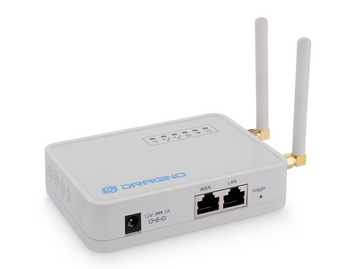
\includegraphics[width=\textwidth]{images/Quanh/lora_gateway.png}
    \caption{LG02 Dragino Gateway} \cite{lg02dragino}
    \label{fig:lorawan_gateway}
\end{figure}

\begin{itemize}
    \item LG02 là open source dual channels LoRa Gateway. Là cầu nối dễ dàng cho LoRa wireless network và IP network: wifi, Ethernet, 3g/4g\dots .
    \item Hỗ trợ giải quyết từ 50-300 sensor nodes
    \item Frequency 433Mhz
\end{itemize}

\section{End-Device}
Kit RF thu phát wifi Blue esp32 + lora sx1278 oled heltec được mô tả như hình \ref{fig:lorawan_kit} với những đặc điểm sau:
\begin{figure}[H]
    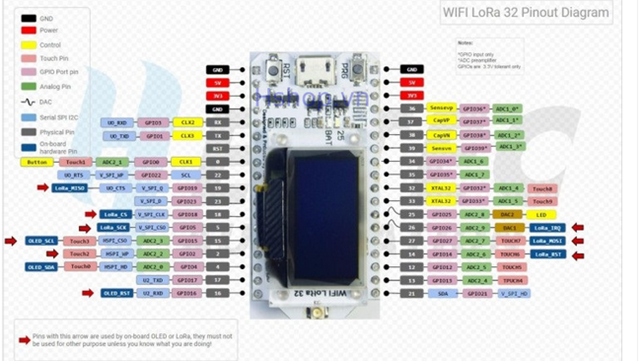
\includegraphics[width=\textwidth]{images/Quanh/lora_kit.png}
    \caption{Kit RF thu phát wifi Blue esp32 + lora sx1278 oled heltec} \cite{lorawan32}
    \label{fig:lorawan_kit}
\end{figure}
\begin{itemize}
    \item Ba chuẩn giao tiếp: wifi, BLE, RF Lora
    \item Frequency 433Mhz
\end{itemize}

\section{Sử dụng Nodejs và Python Server}
Nodejs là nền tảng được xây dựng trên V8 Javascript Engine, được thiết kế để xây dựng các ứng dụng lớn nhỏ và có thể mở rộng nhanh với chi phí ít tốn kém nhất.

Nodejs hoạt động trên một luồng duy nhất sử dụng I/O bất đồng bộ theo hướng sự kiện để duy trì trọng lượng nhẹ và hiệu quả khi đối mặt với các ứng dụng sử dụng nhiều dữ liệu chạy trên các thiết bị phân tán. Vì thế, nó tỏa sáng trong các ứng dụng mạng thời gian thực nhanh, và vì có khả năng xử lý một số lượng lớn các kết nối đồng thời với thông lượng cao, nó cho phép hàng chục nghìn kết nối đồng thời giữa máy khách và máy chủ được trao đổi dữ liệu tự do qua tương đương với khả năng mở rộng cao.

Python là ngôn ngữ lập trình hướng đối tượng đa dạng, sở hữu cấu trúc dữ liệu cấp cao và hệ thống thư viện lớn, được sử dụng linh hoạt vào nhiều mục đích như lập trình ứng dụng web, khoa học và phân tích dữ liệu, tạo nguyên mẫu phần mềm, ...

Việc sử dụng để tính toán nặng đòi hỏi nhiều tài nguyên CPU như Machine Learning hoặc Big Data không phải thế mạnh của Nodejs. Nên sử dụng Python sẽ phù hợp nhất với các dự án dựa trên AI và máy học vì tính đơn giản, linh hoạt và nhất quán, cũng như quyền truy cập vào nhiều thư viện và frameworks phong phú liên quan đến máy học, phân tích dữ liệu và tính toán khoa học, trực quan dữ liệu, ....

\section{Giới thiệu về LSTM và bài toán dự đoán chuỗi dữ liệu đa bước thời gian}
LSTM (Long Short-Term Memory) là phiên bản mở rộng của mạng RNN (Recurrent Neural Network), được thiết kế để giải quyết các bài toán về phụ thuộc dài hạn (long-term dependencies) trong mạng RNN do bị ảnh hưởng bởi vấn đề gradient biến mất.

Mạng LSTM có thể bao gồm nhiều LSTM memory cell liên kết với nhau và kiến trúc cụ thể của mỗi tế bào được biểu diễn như hình \ref{tab.lstm_cell}. Ý tưởng của mạng LSTM là bổ sung thêm trạng thái bên trong tế bào (cell internal state) $s_t$ và ba cổng sàng lọc các thông tin đầu vào và đầu ra cho tế bào bao gồm forget state $f_t$ (loại bỏ thông tin nhận được không cần thiết ra khỏi cell), input gate $i_t$ (chọn lọc thông tin cần thiết thêm vào cell) và output gate $o_t$ (xác định thông tin nào từ cell được sử dụng như đầu ra). Tại mỗi bước thời gian t, các cổng đều lần lượt nhận giá trị đầu vào $x_t$ (đại diện cho một phần tử trong chuỗi đầu vào), sau đó dựa trên cơ chế hoạt động của cell, đưa qua quá trình lan truyền xuôi (forward pass) và giá trị $h_{t-1}$ có được từ đầu ra của memory cell từ bước thời gian trước đó t - 1.

\begin{figure}[H]
    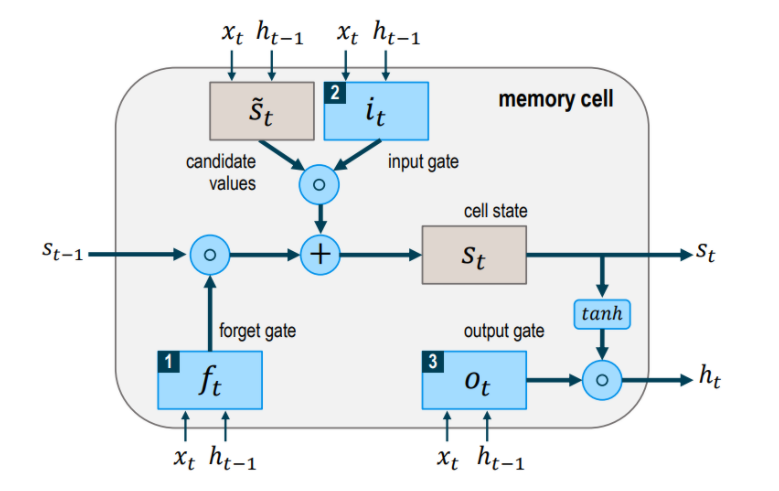
\includegraphics[width=\textwidth]{images/Khanh/Python/LSTM_cell_structure.PNG}
    \caption{Sở đồ biểu diễn kiến trúc bên trong tế bào LSTM} \cite{lstmintroduction}
    \label{tab.lstm_cell}
\end{figure}

Dự đoán trước nhiều bước thời gian là công việc dự đoán một chuỗi các giá trị trong một chuỗi thời gian bằng việc áp dụng mô hình dự đoán từng bước và sử dụng giá trị dự đoán của bước thời gian hiện tại để xác định giá trị của nó trong bước thời gian tiếp theo. Hiện nay có ít nhất bốn chiến lược thường được sử dụng để giải quyết bài toán này:
\begin{itemize}
    \item Dự báo trực tiếp:
    \begin{itemize}
        \item Liên quan đến việc phát triển mô hình riêng biệt cho từng bước thời gian.
        \item Không thích hợp trong việc tính toán và bảo trì vì số lượng bước thời gian dự đoán đôi khi sẽ lên rất nhiều.
        \item Không có cơ hội để mô hình hóa sự phụ thuộc giữa các dự đoán.
    \end{itemize}
    \item Dự báo đệ quy:
    \begin{itemize}
        \item Liên quan đến việc sử dụng mô hình một bước nhiều lần trong đó dự đoán cho bước thời gian trước được sử dụng làm đầu vào để đưa ra dự đoán cho bước thời gian sau.
        \item Cho phép tích lũy các lỗi dự đoán để hiệu suất có thể nhanh chóng suy giảm khi thời gian dự đoán tăng lên.
    \end{itemize}
    \item Dự báo kết hợp:
    \begin{itemize}
        \item Kết hợp giữa trực tiếp và đệ quy để cung cấp các lợi ích của cả hai phương pháp và khắc phụ hạn chế của mỗi chiến lược.
        \item Phát triển mô hình cho từng bước thời gian dự đoán, nhưng mỗi mô hình có thể sử dụng các bước dự đoán được thực hiện bởi các mô hình ở các bước thời gian trước đó làm giá trị đầu vào.
    \end{itemize}
    \item Dự báo nhiều đầu ra:
    \begin{itemize}
        \item Liên quan đến việc phát triển một mô hình có khả năng dự đoán toàn bộ chuỗi dự báo theo cách một lần.
        \item Phức tạp hơn vì chúng có thể tìm hiểu cấu trúc phụ thuộc giữa đàu vào và đầu ra cũng như giữa các đầu ra.
        \item Mô hình đào tạo sẽ chậm hơn và yêu cầu nhiều dữ liệu hơn để tránh Overfitting cho vấn đề.
    \end{itemize}
\end{itemize}

\section{Giới thiệu bài toán TSP (Travelling Salesman Problem)}
TSP (bài toán người du lịch) là một bài toán tối ưu tổ hợp thuộc lớp phức tạp NP-hard, trình bày vấn đề: "Cho sẵn danh sách các thành phố và khoảng cách giữa những thành phố đó, tìm đường đi khả thi ngắn nhất từ điểm bắt đầu đến các thành phố và quay lại điểm bắt đầu, với điều kiện mỗi thành phố chỉ được đi qua một lần". 

Hiện tại đã có nhiều phương pháp giải quyết bài toán này thông qua các thuật toán chính xác, heuristic:
\begin{itemize}
    \item The Brute-Force Approach: Tính toán và so sánh tất cả các hoán vị có thể có của các tuyến đường để xác định đường đi ngắn duy nhất.
    \item The Branch and Bound Method: Tách bài toán lớn thành các bài toán nhỏ theo dạng nhánh, mỗi nhánh sẽ được tính toán và kiểm tra dựa trên các giới hạn ước tính trên và dưới và đưa ra giải pháp riêng. Những giải pháp sẽ được loại bỏ nếu nó không tốt hơn giải pháp tốt nhất được tìm thấy cho đến nay. 
    \item The Nearest Neighbor Method: Chọn tuyến đường bắt đầu và đến những tuyến đường gần nhất của nó và sau đó quay trở về khi nó đã đến hết tất cả tuyến đường trên bản đồ. 
\end{itemize}
Ngoài ra, nhiều giải pháp học thuật cũng được đưa ra để giải quyết những vấn đề phụ mà các phương pháp phổ biến hiện nay đang gặp phải: Zero Suffix Method, Biogeography-based Optimization Algorithm, Multi-Agent System, Multi-Objective Evolutionary Algorithm, ... 

Về mặt lý thuyết, việc giải quyết TSP sẽ dễ dàng hơn vì bạn phải tìm ra con đường ngắn nhất cho mỗi chuyến đi trong thành phố. Nhưng nó trở nên khó khăn để giải quyết TSP bằng tay khi số lượng thành phố tăng lên, bất kì giải thuật nào cho bài toán TSP cũng sẽ tăng theo hàm mũ với số lượng thành phố. Ngoài ra, một số ràng buộc làm cho TSP khó giải quyết hơn (giao thông, thay đổi tuyến đường đột ngột, phương tiện di chuyển,...). Vì thế trong lý thuyết của độ phức tạp tính toán, phiên bản quyết định của bài toán TSP thuộc lớp NP-Complete, tức là không có giải thuật hiệu quả duy nhất nào cho việc giải bài toán. 

\section{Giới thiệu về Mapbox}
Mapbox là nền tảng đám mây hỗ trợ định vị và xử lý dữ liệu bản đồ thông qua các API dễ dàng tích hợp vào trang web hoặc ứng dụng của mình với giá cả rất hợp lý. Không những thế, Mapbox cho phép sử dụng miễn phí API tối đa ở 100.000 request 1 API, vì thế nâng cao trải nghiệm của người lập trình cho đến khi họ thực sự muốn xài dịch vụ.

Mapbox sở hữu một trang docs với tất cả các API hỗ trợ từ vẽ, thiết kế bản đồ, quản lý các điểm, cho đến hỗ trợ tìm đường nhanh, ma trận đường, geocoding, ... Vì để giải quyết bài toán thu gom rác trong dự án, Mapbox API, cụ thể là Route-matrix và Optimization API sẽ được sử dụng để tìm thời gian đi và đường đi tối ưu nhất từ một điểm đến các điểm còn lại. 

\section{Giới thiệu về Thingsboard}
Thingsboard là một nền tảng IoT mã nguồn mở, giúp phát triển, quản lý và mở rộng các dự án về Iot. Với Thingsboard, việc thu thập, xử lý, hiển thị trực quan và quản lý thiết bị sẽ trở nên thuận lợi hơn thông qua việc kết nối các thiết bị bằng các giao thức IoT tiêu chuẩn công nghiệp - MQTT, CoAP và HTTP, hỗ trợ triển khai đám mây và tại chỗ. Ngoải ra, Thingsboard cho phép tích hợp các thiết bị được kết nối với các máy chủ (OPC-UA, MQTT Broker, Sigfox Backend, Modbus slaves, ...) và bên thứ ba qua IoT Gateway bằng các giao thức hiện có (Sigfox, LoRa, ZigBee, Bluetooth, ...). Hình \ref{fig:thingsboard_overall} hiển thị mô hình tổng quát của Thingsboard

\begin{figure}[h]
    \centering
    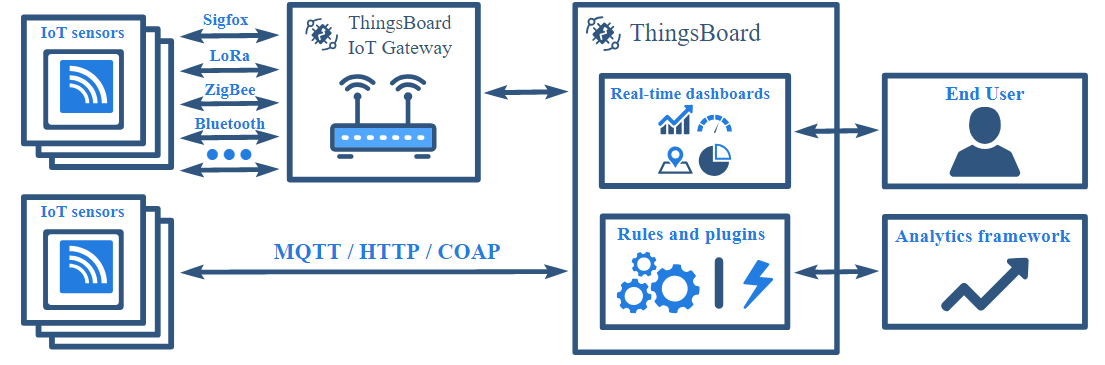
\includegraphics[width=\textwidth]{images/Khanh/Thingsboard/thingsboard_overall.png}
    \caption{Mô hình tổng quan Thingsboard} \cite{thingsboard}
    \label{fig:thingsboard_overall}
\end{figure}

Với các tính năng ưu việt như thu thập dữ liệu từ xa, quản lý thiết bị và các báo động, Thingsboard cung cấp hơn 30 tiện ích có sẵn (Google map, Realtime chart, HTML tab, ...), cho phép tạo các bảng điều khiển (Dashboard) phong phú để hiển thị trực quan dữ liệu và điều khiển từ xa trong thời gian thực.

Bên cạnh đó, Thingsboardcho phép tạo các chuỗi quy tắc (Rule chains) kéo thả thân thiện để xử lý dữ liệu thiết bị dựa trên thuộc tính thực thể hoặc nội dung tin nhắn, tùy chỉnh logic xử lý phù hợp với các trường hợp sử dụng ứng dụng cụ thể. 


